\documentclass[11pt, letterpaper]{elsarticle}
\usepackage{amsmath}
\usepackage{amssymb}
\usepackage{tikz}
\usepackage{tikz,fullpage}
\usepackage{pgf}
\usepackage{pgfplots}
\usetikzlibrary{
	pgfplots.fillbetween,
}
\usetikzlibrary{arrows,automata}
\usepackage{tkz-berge}

\begin{document}

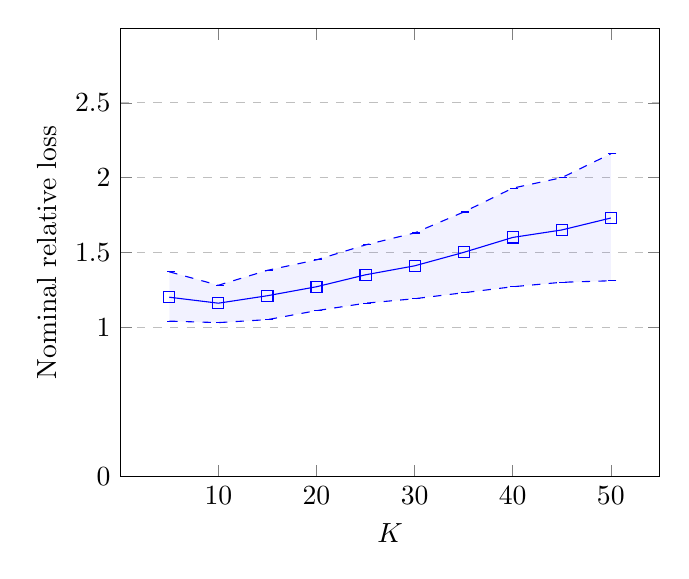
\begin{tikzpicture}
	\begin{axis}[
	xlabel={$K$},
	ylabel={Nominal relative loss},
	xmin=0, xmax=55,
	ymin=0, ymax=3,
	xtick={10,20,30,40,50},
	ytick={0,1,1.5,2,2.5},
	legend pos=north west,
	ymajorgrids=true,
	grid style=dashed,
	]
	
	\addplot[name path=f1,
	color=blue,
	mark=square,
	]
	coordinates {
		(5,	1.20)
		(10,	1.16)
		(15,	1.21)
		(20,	1.27)
		(25,	1.35)
		(30,	1.41)
		(35,	1.50)
		(40,	1.60)
		(45,	1.65)
		(50,	1.73)
	};
	
	\addplot[name path=f2,
	color=blue,
	style=dashed,
	mark=-,
	]
	coordinates {
		(5,	1.04)
		(10,	1.03)
		(15,	1.05)
		(20,	1.11)
		(25,	1.16)
		(30,	1.19)
		(35,	1.23)
		(40,	1.27)
		(45,	1.30)
		(50,	1.31)
		};
	\addplot[name path=f3,
	color=blue,
	style=dashed,
	mark=-,
	]
	coordinates {
		(5,	1.37)
		(10,	1.28)
		(15,	1.38)
		(20,	1.45)
		(25,	1.55)
		(30,	1.63)
		(35,	1.77)
		(40,	1.93)
		(45,	2.00)
		(50,	2.16)
	};
	
		\addplot [
	thick,
	color=blue,
	fill=blue, 
	fill opacity=0.05
	]
	fill between[
	of=f3 and f2,
	soft clip={domain=5:50},
	];
    \end{axis}
	\end{tikzpicture}

\end{document}